\section{Formal Mapping to IFGT and VED}


This section maps the consciousness model of this paper onto the IFGT and VED framework.

The aim is not to reduce consciousness to a physical field, nor to map brain phenomena directly onto cosmological equations.

The purpose is to fix a minimal correspondence that allows consciousness to be read as a local, projected implementation of information flow, meaning potential, and non-closure dynamics.

\subsection{Projected Uses and the Projection Operation}
\label{sec:projected-uses}

Before introducing the IFGT mapping in the following subsections, this
subsection fixes the methodological status of the vocabulary used
throughout this paper and the structural definition of projection as
the fourth IFGT primitive.

The reason for placing this discussion before the IFGT mapping is
simple. Whenever the variables \(I\), \(J_I\), \(\Phi\), and the local
flow \(J_{\mathrm{log}}\) are introduced, two distinct questions are
present at once: \emph{what these variables refer to in a general IFGT
field}, and \emph{how this paper uses them inside a biological--cognitive
observation window}. Conflating the two readings has caused recurring
misunderstandings of consciousness models built on field-theoretic
vocabularies. The position of this paper is fixed in advance, here.

\subsubsection{The Position: Projected Uses}
\label{sec:projected-uses-stance}

In this paper, the IFGT variables are used not as direct identifications
with a general information field, but as \emph{projected} variables
inside a specific observation window.

Concretely:

\begin{itemize}
  \item \(I\), \(J_I\), and \(\Phi\) appear in this paper as effective
        coordinates within the biological--cognitive window, not as the
        full IFGT field itself.
  \item The local log-referencing flow \(J_{\mathrm{log}}\) is treated as
        a window-local flow variable, not as a global IFGT current.
  \item Equations involving these variables are read as descriptions of
        \emph{this} window, not as ontological claims about a universal
        information field.
\end{itemize}

This position is called \emph{projected uses}. It is the same
methodological stance adopted in the parallel intelligence paper
\cite{Intelligence}, and the two papers share this stance as their
common epistemological foundation.

Two consequences follow.

First, the equations in §§7--9 do not claim to be universal field
equations of consciousness. They are structural relations holding within
the biological--cognitive window in which consciousness is described in
this paper.

Second, when this paper speaks of correspondence with VED, Bio-IFGT,
Conceptual Topography (CT), or the intelligence paper, the
correspondence is read as a relation between \emph{different projected
windows of the same underlying differential-development structure}, not
as a reduction of one description to another. No paper grounds another;
each is a window-local description.

\subsubsection{Projection as the Fourth IFGT Primitive}
\label{sec:projection-definition}

In addition to information density \(I\), information flow \(J_I\), and
information potential \(\Phi\), this paper uses a fourth structural
primitive: \emph{projection}, in the sense of \emph{mass assignment}.

\paragraph{Definition.}
\emph{Projection} is the operation by which a specific state or
representation acquires disproportionate influence within the dynamics.

\begin{itemize}
  \item Projection is the structural description of attention,
        selection, and prioritization.
  \item Projection does not require intentional choice; physical
        biasing, biological prioritization, and artificial weighting are
        all included.
  \item Projection is the mechanism that couples \(\Phi\) and \(J_I\):
        it is the operation through which a global bias localizes onto
        a specific state.
\end{itemize}

In the language of this paper, the operation that selects which logs
the slow layer reinforces, which fast-layer activity passes through the
plasticity gate, and which direction \(\nabla\Phi\) imposes on
\(J_{\mathrm{log}}\) are all instances of projection at the
biological--cognitive window. The effective torque-like quantity
\(\mathcal{T}_\Phi \sim \kappa (\Delta v / \mu)\,|\nabla\Phi|\)
introduced in §5 and §7 is the structural index of how strongly
projection operates in a given moment of the consciousness window.

Projection therefore plays a load-bearing role in this paper, even
though earlier sections do not name it explicitly. The plasticity gate,
the meaning-gradient bias, the qualia residue selection in §13, and the
referencing-pathway asymmetry in split-brain experiments (§10) are all,
structurally, projection operations under different local conditions.

\subsubsection{Relation to the Psychological Notion of Projection}
\label{sec:projection-disclaimer}

The term \emph{projection} is also used in psychology, particularly in
the psychoanalytic tradition, to mean the mechanism by which a subject
attributes its own internal state to another person or external object.
The terminological overlap with the present usage is real, but the
structural status is not the same.

The psychological notion of projection presupposes a subject, an
unconscious, and internal states. The IFGT notion of projection used in
this paper presupposes none of these at the axiomatic level. Both
notions share the structural feature of \emph{unequal weight
assignment}, and the psychological notion can be read as an
operational-level instance of IFGT projection at a specific layer:
namely, its concrete manifestation on the surface of complex systems
that possess subjectivity.

Neither concept reduces the other. They describe the same structure at
different granularities. The present paper restricts itself to the
structural level, and the detailed correspondence with the psychological
concept lies outside its scope. Where the rest of this paper says
``projection,'' the structural sense alone is intended.

\subsubsection{What This Subsection Does Not Claim}
\label{sec:projected-uses-non-claims}

For clarity, two non-claims are stated explicitly.

\begin{itemize}
  \item This subsection does not claim that the consciousness window is
        identical to any specific cross-section of a general IFGT field.
        The relation is one of \emph{projection}, in the sense fixed
        above.
  \item This subsection does not claim that biological--cognitive,
        intelligence-layer, or conceptual-landscape windows are mutually
        reducible. They are described as different projected windows of
        the same differential-development structure, and the question
        of inter-window dynamics is treated elsewhere
        (\cite{Intelligence}, §9.4).
\end{itemize}

With these clarifications, the rest of §6 proceeds to map the
consciousness model onto IFGT and VED in the projected-uses sense fixed
here. The reader should henceforth read \(I\), \(J_I\),
\(J_{\mathrm{log}}\), \(\Phi\), and projection as window-local
structural primitives, not as the full IFGT field.

\subsection{IFGT Mapping: Information, Flow, Potential}


The basic variables of IFGT are information density $I$, information flow $J_I$, information-field potential $\Phi$, and projection (§\ref{sec:projection-definition}).

In the projected-uses sense fixed in §\ref{sec:projected-uses-stance}, this paper uses these variables as effective coordinates within the biological--cognitive window. That is, $I$, $J_I$, and $\Phi$ are not direct identifications with a general IFGT field, but window-local effective coordinates for describing log sedimentation, log referencing, and meaning-gradient bias. Projection operates throughout the mapping below as the operation coupling these variables under the structural definition fixed in §\ref{sec:projected-uses}.

In this paper, the elements of the consciousness model are mapped as follows:

\begin{itemize}
\item $I$: density of logs sedimented in the slow layer.
\item $J_{\log}$: processing flow from the fast layer toward the slow layer, or the flow of log referencing.
\item $\Phi$: information potential formed by log configuration — the meaning field.
\item $\nabla\Phi$: meaning gradient that directs which logs are easily referenced.
\item $\partial\Phi/\partial t$: live change in the meaning field.
\end{itemize}

$I$ is not merely a quantity of memory.

It is the density of logs sedimented in a re-referenceable form.

$J_{\log}$ is not merely information transmission.

It is the dynamic flow expressing which logs current processing moves toward, which it updates, and into which meaning wells it flows.

$\Phi$ does not represent meaning inhering in the logs.

Meaning is not stored within logs; it is established as a potential formed by the configuration of logs in relation to one another.

Log referencing in a conscious state is therefore not merely the retrieval of stored content from the slow layer.

It is the process by which current fast processing connects to the slow layer along the gradient of the existing information potential.

\subsection{IFGT Core Relations}


The minimal relations of IFGT are given in the following form:

\begin{equation}
\frac{\partial I}{\partial t} + \nabla \cdot J_I = \sigma
\end{equation}

\begin{equation}
J_I = -D \nabla I + \mu_I F
\end{equation}

\begin{equation}
F = -\nabla \Phi
\end{equation}

\begin{equation}
\Phi = K * I
\end{equation}

Here $\sigma$ is the generation-dissipation term for information density, $D$ is the diffusion coefficient, $\mu_I$ is the mobility of information flow, $F$ is the effective force arising from the information potential, and $K$ is the kernel giving the potential from information density.

In this paper, these are not used as completed equations of consciousness.

They are the structural template for describing in which projected field log referencing is directed.

That is: consciousness is not $I$ itself, not $J_I$ itself, not $J_{\log}$ itself, and not $\Phi$ itself.

Consciousness is the state that opens when information density, information flow, and information potential become interconnected within a processing system with a time-scale difference.

\subsection{VED Mapping: Non-Closure as Condition}


The foundation of VED is a dynamic structure that does not treat complete closure as an ordinary attainable state.

There is difference, gradient forms, flow arises, and structure tends toward closure; complete closure, however, is not realized as an ordinary generated state.

This non-closure is the condition for the persistence of motion.

The same structure appears in the consciousness model.

If the fast and slow layers fully synchronize, the speed difference $\Delta v$ vanishes:

\begin{equation}
\Delta v \rightarrow 0
\end{equation}

Processing then smoothly automates, but the boundary for log referencing disappears.

Conversely, if the fast and slow layers fully separate, flow $J_{\log}$ does not reach the slow layer. Processing occurs, but does not sediment as a referenceable log.

Conscious state is therefore neither complete synchrony nor complete separation.

It is a non-closure regime in which difference persists, flow is maintained, and yet no rupture occurs.

This minimal condition is written:

\begin{equation}
\Delta v \neq 0
\end{equation}

This does not mean that a larger speed difference is better.

What is required is that a finite speed difference is maintained without rupture through the coupling viscosity $\mu$.

In this sense, SSO is the local temporal non-closure structure in the brain.

\subsection{VED Closure Degree and the SSO Window}


This subsection is an auxiliary mapping for readers who require the VED-side formalization.

For intuitive understanding, it is sufficient to read $\Delta v$ as a time-scale difference.

In VED, the closure degree between any two nodes $i, j$ is defined as:

\begin{equation}
C_{ij} = 1 - \exp\!\left(-\lambda \rho_i H_{ij}\right)
\end{equation}

Here $\rho_i$ is the density of difference at node $i$, $H_{ij}$ is the connection strength between nodes, and $\lambda$ is a scale factor.

$C_{ij} \to 1$ corresponds to the complete-closure boundary: difference vanishes, flow stops, and the generated description loses the distinction on which it depends.

$C_{ij} \to 0$ corresponds to complete non-closure: no connection is established between nodes.

The mapping to the consciousness model proceeds as follows.

Let $C_f$ denote the effective closure degree of the fast layer and $C_s$ that of the slow layer.

The fast layer is predictive and volatile, so closure does not readily advance; $C_f$ maintains a relatively low value.

The slow layer is sedimentary and stable, so closure advances more readily; $C_s$ tends to take higher values than $C_f$.

From this asymmetry, the closure degree difference is defined as:

\begin{equation}
\Delta C = C_s - C_f
\end{equation}

This $\Delta C$ is the structural quantity corresponding to the speed difference $\Delta v$ used throughout this paper:

\begin{equation}
\Delta v \;\leftrightarrow\; \Delta C
\end{equation}

That is, speed difference was introduced as "difference in processing time scales"; in the language of VED it is read as "difference in closure degree between the two layers."

The window condition for a conscious state to obtain is written in terms of closure degree difference as:

\begin{equation}
0 < \Delta C < \Delta C_{\max}
\end{equation}

$\Delta C = 0$ corresponds to complete synchrony: fast and slow layers reach the same closure degree and the boundary for referencing disappears.

$\Delta C \to \Delta C_{\max}$ corresponds to referencing disconnection: the divergence in closure degree is too large and fast-layer processing can no longer reach the slow layer.

The consciousness window is thus expressed, in the language of VED, as the closure-degree-difference regime in which $\Delta C$ maintains a finite nonzero value.

Furthermore, the older VED non-closure persistence condition

\begin{equation}
\frac{\partial C}{\partial t} + \nabla \cdot J_C = a\Delta\!\left(1 - C/C_*\right) - \Gamma C - \frac{\kappa_B}{C_{\max} - C}
\end{equation}

is read in the consciousness model as a phenomenological, coarse-grained approximation.

The first term $a\Delta(1 - C/C_*)$ represents the tendency toward closure driven by difference. It corresponds to the force by which the fast layer draws the slow layer toward it.

The second term $-\Gamma C$ represents dissipation against excessive closure advance. It is the term that prevents complete synchrony, providing the condition that prevents speed difference from vanishing.

The third term $-\kappa_B/(C_{\max} - C)$ represents a phenomenological effective barrier that grows as closure approaches saturation. In the revised Vol.4 interpretation, this should not be read as a fundamental external prohibition. It is a projected resistance term summarizing the fact that complete closure cannot be realized as an ordinary state inside the generated description.

Through this three-term structure, SSO self-sustainingly maintains the intermediate regime that reaches neither complete closure nor complete separation.

This is the VED-grounded basis for the non-closure persistence condition of the conscious state.

Figure~\ref{fig:sso-ved-mapping} shows the structural correspondence between the SSO and VED descriptions.

\begin{figure}[H]
\centering
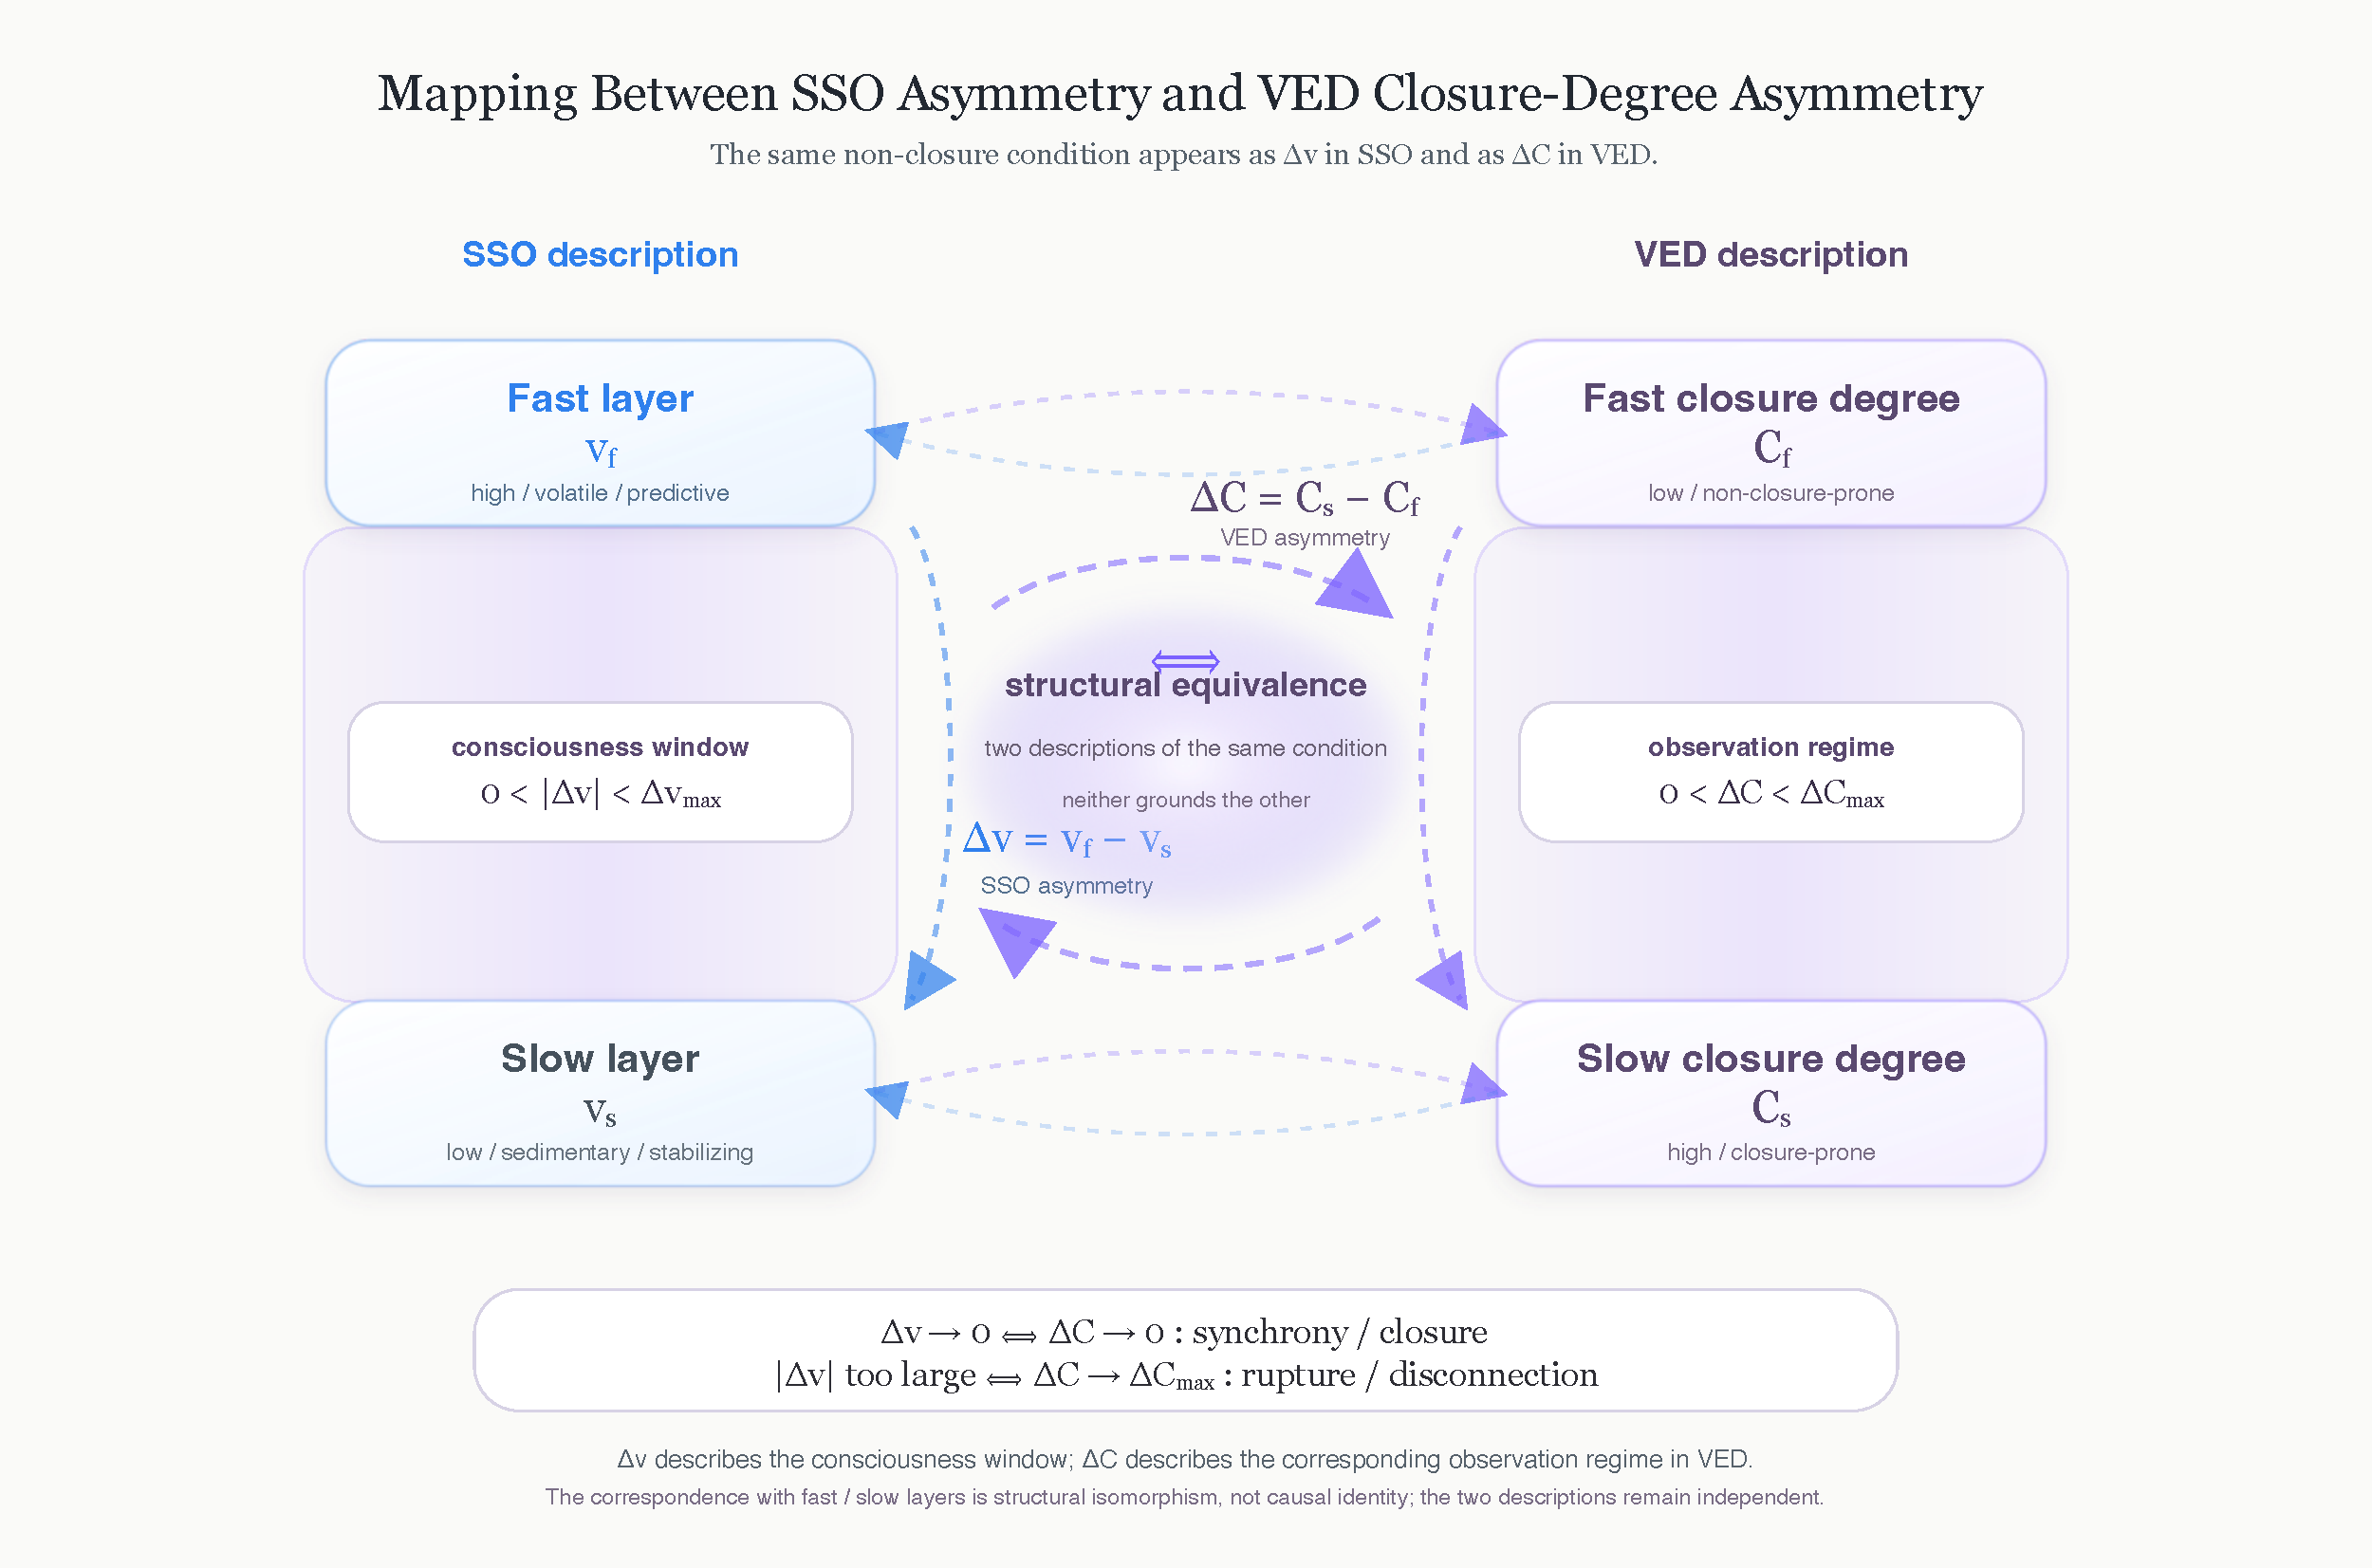
\includegraphics[width=0.94\linewidth]{figures/figure6_observation_regime.pdf}
\caption{
Mapping between SSO asymmetry and VED closure-degree asymmetry.
The speed difference \(\Delta v\) in SSO and the closure-degree difference \(\Delta C = C_s - C_f\) in VED describe the same non-closure condition in different coordinates.
The consciousness window on the SSO side corresponds structurally to the observation regime on the VED side, without either description grounding the other.
}
\label{fig:sso-ved-mapping}
\end{figure}

\subsection{SSO as Local Non-Closure}


SSO (Speed-Scale Orchestration) is a structure in which processes at multiple time scales are coordinated without central control.

From the VED perspective, SSO is a local model of a temporal structure that does not close completely.

The fast layer predicts; the slow layer sediments.

The fast layer advances; the slow layer fixes with a lag.

This difference is not eliminated.

Rather, it is because this difference remains that a referencing relation arises between current processing and past logs.

The conditions for SSO to obtain are three:

\begin{enumerate}
\item Speed difference between fast and slow layers exists.
\item The two layers are not completely separated.
\item Sedimentation into the slow layer has not closed completely.
\end{enumerate}

When these three conditions are met, processing does not merely flow away into the present but opens a relation to past logs.

Here the conscious state as log referencing obtains.

\subsection{Torque Converter Attention as IFGT/VED Coupler}


Torque Converter Attention is the point of connection between IFGT and VED.

From the VED perspective, it is a non-closure mechanism that transmits speed difference $\Delta v$ without eliminating it.

From the IFGT perspective, it is a mechanism that adjusts, along the gradient of the information potential $\Phi$, which logs are easily referenced.

For this reason, the effective torque-like quantity $\mathcal{T}$ is first expressed through speed difference and coupling viscosity:

\begin{equation}
\mathcal{T} = \kappa \frac{\Delta v}{\mu}
\end{equation}

However, in a conscious state, which logs are referenced is not determined by speed difference alone.

Log referencing is directed by the meaning gradient.

The effective quantity in the consciousness model is therefore extended to include the gradient of the information potential:

\begin{equation}
\mathcal{T}_{\Phi} \sim \kappa \frac{\Delta v}{\mu} |\nabla \Phi|
\end{equation}

Here $\mathcal{T}_{\Phi}$ is the effective torque-like quantity in which time-scale difference and meaning gradient are coupled.

This is not a quantity that generates consciousness.

It is a structural index showing how strongly and in which direction log referencing tends to open.

\subsection{Consciousness as IFGT/VED Interface}


On the basis of the above, consciousness in this paper is positioned as a local projected regime at the interface between IFGT and VED.

IFGT provides the configuration of logs, meaning field, and information flow.

VED provides the condition by which that configuration does not realize complete closure as an ordinary state, maintaining difference and flow.

Consciousness is modeled where these two descriptions overlap.

That is, consciousness is the state in which log referencing directed by the projected information potential is open within a temporal non-closure regime that reaches neither complete synchrony nor complete separation.

In minimal form:

\begin{equation}
\text{Consciousness} \sim \text{Log Referencing}\!\left(I, J_{\log}, \Phi, \Delta v, \mu, \tau, \mathcal{T}_{\Phi}\right)
\end{equation}

This expression does not compute consciousness.

It is the coordinate showing the structural variables required when speaking of consciousness.

Consciousness is not reducible to $I$ alone, nor to $J_I$, $J_{\log}$, $\Phi$, or $\Delta v$ alone.

Consciousness opens when these are coupled within a state of temporal non-closure.

\paragraph{Positioning as a Projection of the Differential-Development Structure}
The position of consciousness fixed in this section at the IFGT/VED interface
is placed within a broader structure. VED describes the physical layer,
Bio-IFGT the biological layer, this paper the consciousness layer, and the
intelligence paper~\cite{Intelligence} the intelligence layer. These four
layers repeat the same differential-development structure at different
granularities, and each paper describes one of its projected windows. The
projected-uses stance fixed in §\ref{sec:projected-uses-stance} requires that
the relations among these multiple windows be read not as "mutual reduction"
but as "different projections of the same structure." The detailed
correspondence between the consciousness window of this paper and the other
layers is organized in §20.

\subsection{Why This Mapping Is Minimal}


The mapping in this section is deliberately held to a minimum.

There are two reasons.

First, over-formalizing consciousness carries the risk of treating it as a closed object. But in the position of this paper, consciousness is not a completely closed object; it is a non-closed log-referencing state.

Second, the role of IFGT/VED is not to explain consciousness completely but to place the question of consciousness in the correct position.

This section therefore does not provide a unified equation of consciousness.

What it provides is the minimal correspondence showing between which variables consciousness opens.

This minimal mapping allows the paper to organize the core equations in the next section — handling speed difference, coupling viscosity, internal delay, effective torque-like quantity, meaning gradient, and non-closure condition within a single structure.
